\documentclass[10pt,openany]{book}
\usepackage[top=2cm,bottom=2cm,left=2cm,right=2cm,letterpaper]{geometry}
\usepackage{emptypage}
\usepackage[utf8]{inputenc}
\usepackage{steinmetz}
\usepackage{amssymb}
\usepackage{mathrsfs}
\usepackage{amsmath}
\usepackage{parskip}
\usepackage{scalerel}
\usepackage{sectsty}
\usepackage{graphicx}
\usepackage[spanish,es-noshorthands]{babel}
\usepackage[svgnames,dvipsnames,x11names,table]{xcolor}
\usepackage[listings,many]{tcolorbox,empheq}
\usepackage{colortbl}
\usepackage{booktabs}
\usepackage{lmodern}
\usepackage{utopia}
\usepackage[shortlabels]{enumitem}
\usepackage{tikz,tkz-euclide,pgf}
\usepackage{pgfplots}
\usepackage{array}
\usepackage[american voltages]{circuitikz}
\usepackage{float}
\usepackage{wrapfig}
\usepackage{varwidth}
\usepackage{latexsym}
\usepackage{caption}
\usepackage{subfigure}
\usepackage{multicol}
\usepackage[explicit]{titlesec}
\usepackage{titletoc}
\usepackage{etoolbox}
\usepackage{framed}
\usepackage{fancyhdr}
\usepackage{rotating}
\usepackage{pdfpages}
\usepackage{hyperref}
\usepackage{multirow}
\usepackage[dvipsnames]{xcolor}

\pagestyle{plain}

\spanishdecimal{.}

\raggedbottom

\begin{document}

\input{Portada.tex}

\tableofcontents

\newpage
\section*{Objetivos}
\addcontentsline{toc}{section}{Objetivos}
\begin{itemize}
    \item Entrenar al estudiante en la utilización y manipulación del osciloscopio. 
    \item Determinar la resistencia interna de una fuente de alimentación o generador. 
    \item Llevar a cabo la edición de la constante de tiempo de redes eléctricas de primer orden pasa bajas.
    \item Realizar la medición de los parámetros de diseño de una red eléctrica de segundo orden, a partir de la respuesta al escalón.
    \item Encontrar el valor de los elementos que constituyen una red eléctrica, a partir de las mediciones anteriores.
\end{itemize}

\section*{Introducción}
\addcontentsline{toc}{section}{Introducción}
La teoría de circuitos eléctricos se basa en la representación y análisis de sistemas de primer y segundo orden. 

\subsection*{Sistemas de Primer Orden}
\addcontentsline{toc}{subsection}{Sistemas de Primer Orden}
Un sistema de primer orden tiene una función de transferencia de la forma:
\begin{equation}
    H(s) = \frac{M}{\tau s + 1}
\end{equation}
La respuesta al escalón se expresa como:
\begin{equation}
    yzs(t) = M k \left(1 - e^{-t/\tau} \right)
\end{equation}
La constante de tiempo $\tau$ es el tiempo que toma alcanzar el 63.2\% del valor final.

\subsection*{Sistemas de Segundo Orden}
\addcontentsline{toc}{subsection}{Sistemas de Segundo Orden}
Un sistema de segundo orden tiene una función de transferencia:
\begin{equation}
    H(s) = \frac{\omega_n^2}{s^2 + 2\zeta \omega_n s + \omega_n^2}
\end{equation}
Dependiendo del coeficiente de amortiguamiento $\zeta$, se tienen diferentes respuestas al escalón.

\section*{Desarrollo Experimental}
\addcontentsline{toc}{section}{Desarrollo Experimental}

\subsection*{Experimento 1. Medición de la resistencia interna del generador, $r_g$.}
\addcontentsline{toc}{subsection}{Experimento 1: Medición de la resistencia interna del generador, $r_g$.}
\begin{figure}[h]
    \centering
    \begin{circuitikz}
        \draw (3,0) to [short, *-] (6,0) 
            to [R, l_=$R\mathord{=}500\Omega$] (6,3)
            to [short, -] (6,3)
            to [closing switch, l_=$S$, mirror, invert] (4,3)
            to [short, -*] (3,3)
            to [open, v^>=$v$] (3,0)
            to [short, -] (0,0)
            to [V, v=$v_g\mathord{=}E$,  invert] (0,3)
            to [short, -] (0,3)
            to [R, l=$r_g$] (2,3)
            to [short, -*] (3,3);
    \end{circuitikz}
    \caption{Circuito el´ectrico para determinar la resistencia interna del generador, $r_g$.}
    \label{fig:circuito1}
\end{figure}
Construya el circuito eléctrico de la figura 1. La resistencia interna del generador, $r_g$ se puede determinar por medio de la ecuación
\[
    \frac{\text{Amplitud de }v\text{ con }S\text{ cerrado}}{\text{Amplitud de }v\text{ con }S\text{ abierto}} = \frac{R}{r_g + R}
\]

\subsection*{Experimento 2: Medición de la inductancia del inductor.}
\addcontentsline{toc}{subsection}{Experimento 2: Medición de la inductancia del inductor.}

Mida la resistencia RL del inductor. A continuación, construya el circuito eléctrico de la figura 2. Ajuste la amplitud
$A$ y la frecuencia $f$ de la señal cuadrada del generador de funciones de tal forma que en el osciloscopio se visualice
la respuesta al escalón del circuito RL.
\begin{figure}[h]
    \centering
    \begin{circuitikz}
        \draw (5,0) to [short, -*] (6,0) 
            to [open, v^<=$v_0$] (6,4)
            to [short, *-] (5,4)
            to [R, l_=$R\mathord{=}500\Omega$] (5,0)
            to [short, -] (0,0)
            to [V, l=$v_g$, invert] (0,2)
            to [R, l=$r_g$] (0,4)
            to [L, l=$L$] (2,4) 
            to [R, l=$r_L$] (4,4)
            to [short, -] (5,4);
    \end{circuitikz}
    \caption{Circuito eléctrico RL.}
    \label{fig:circuito2}
\end{figure} 
\begin{enumerate}[a)]
    \item Con el auxilio del osciloscopio, determine experimentalmente el valor de la constante de tiempo $\tau$.
    \item Con el valor de $\tau$ , encuentre el valor de la inductancia del inductor.
\end{enumerate}
\color{BlueViolet}
La inductancia se calcula como:
\[
    \tau = \frac{L}{R}
\]
\color{black}
\subsection*{Experimento 3: Capacitancia de un Capacitor}
\addcontentsline{toc}{subsection}{Experimento 3: Capacitancia de un Capacitor}
Construya el circuito eléctrico de la figura 6, ajuste la amplitud $A$ y la frecuencia $f$ de la señal cuadrada del
generador de funciones de tal forma que en el osciloscopio se visualice la respuesta al escalón del circuito RC,
semejante a la que se muestra en la figura 1.
\begin{figure}[h]
    \centering
    \begin{circuitikz}
        \draw (5,0) to [short, -*] (6,0) 
            to [open, v^<=$v_0$] (6,4)
            to [short, *-] (5,4)
            to [C, l_=$C\mathord{=}0.22\mu F$] (5,0)
            to [short, -] (0,0)
            to [V, l=$v_g$, invert] (0,2)
            to [R, l=$r_g$] (0,4)
            to [R, l=$R\mathord{=}1k\Omega$] (4,4)
            to [short, -] (5,4);
    \end{circuitikz}
    \caption{Circuito eléctrico RC.}
    \label{fig:circuito3}
\end{figure} 
\begin{enumerate}[a)]
    \item Con el auxilio del osciloscopio, determine experimentalmente el valor de la constante de tiempo $\tau$.
    \item Con el valor de $\tau$ , encuentre el valor de la capacitancia del capacitor.
\end{enumerate}
Te\'oricamente:
\begin{eqnarray*}
  \tau = RC = 1000(0.22\times 10^{-4}) = 2.2\times 10^{-4} & \hspace{2cm} C= 0.22\times10^{-6} [F]
\end{eqnarray*}

Simulaci\'on:
\begin{eqnarray*}
\tau = RC = 1050(0.22\times 10^{-4}) = 2.31\times 10^{-4} & \hspace{2cm} C= \frac{2.31\times 10^{-4}}{1050} = 0.22\times10^{-6} [F]
\end{eqnarray*}
\begin{multicols}{2}
    \begin{center}
        \begin{figure}[H]
            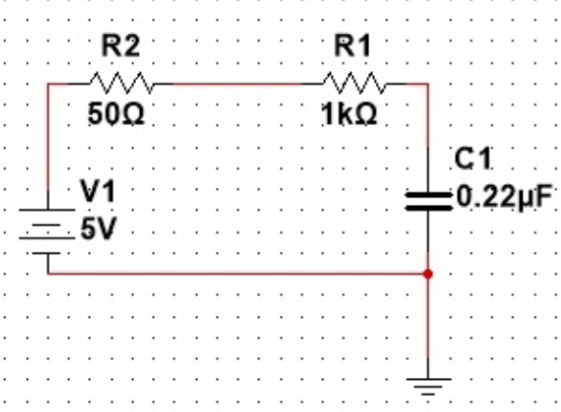
\includegraphics[width=.9\columnwidth]{Figuras\E2a.png}
        \end{figure}
        \begin{figure}[H]
            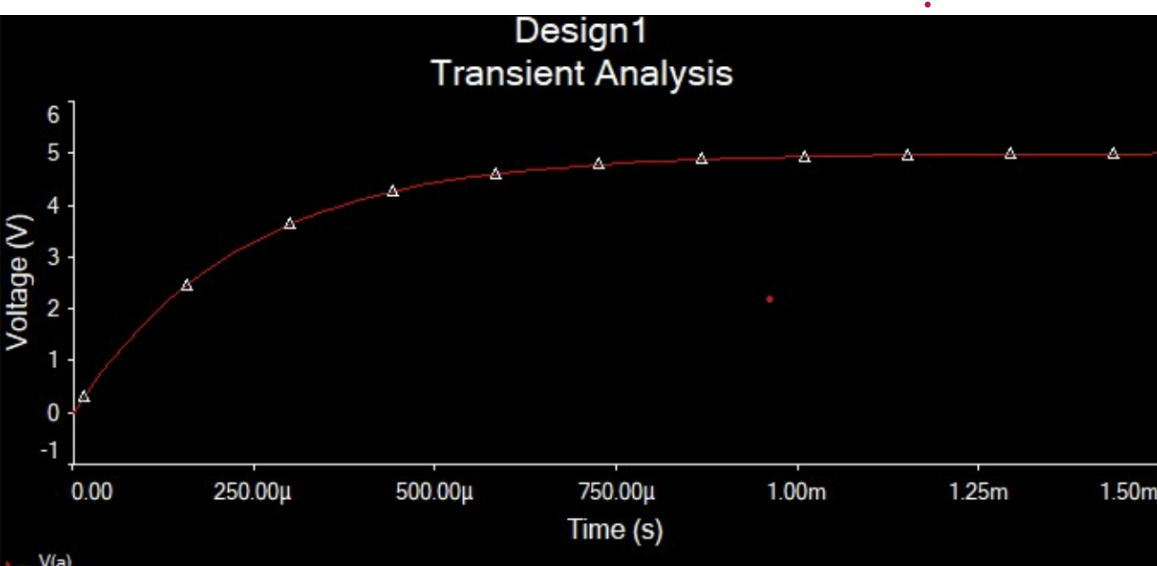
\includegraphics[width=.9\columnwidth]{Figuras\E2b.png}
        \end{figure}
        \end{center}
\end{multicols}
La capacitancia se obtiene con:
\begin{equation}
    \tau = RC
\end{equation}

\newpage
\subsection*{Experimento 4: Sistema eléctrico de segundo orden.}
\addcontentsline{toc}{subsection}{Experimento 4: Sistema eléctrico de segundo orden}
Después de construir el circuito eléctrico de la figura 7, ajuste la amplitud $A$ y la frecuencia $f$ de la señal cuadrada
del generador de funciones de tal forma que en el osciloscopio se visualice la respuesta al escalón del circuito RLC.
\begin{figure}[h]
    \centering
    \begin{circuitikz}
        \draw (5,0) to [short, -*] (6,0) 
            to [open, v^<=$v_0$] (6,4)
            to [short, *-] (5,4)
            to [C, l_=$C$] (5,0)
            to [short, -] (0,0)
            to [V, l=$v_g$, invert] (0,2)
            to [R, l=$r_g$] (0,4)
            to [L, l=$L$] (2,4) 
            to [R, l=$r_L$] (4,4)
            to [short, -] (5,4);
    \end{circuitikz}
    \caption{Circuito eléctrico RLC serie}
    \label{fig:circuito3}
\end{figure}
\\
El inductor y el capacitor son los mismos que se han empleado en los experimentos y calcule teóricamente los parámetros de diseño definidos en las ecuaciones (9), (10), (11), (12) y (13). \\
Determine experimentalmente con el auxilio del osciloscopio, los parámetros calculados previamente. A continuación escriba sus resultados en la Tabla 1. \\
\begin{center}
    \begin{tabular}{| c | c | c |}
        \hline
        \multicolumn{3}{| c |}{Tabla 1} \\ \hline
        Especificación de diseño & Teórico & Experimental \\ \hline
        $M_p$ &  &  \\ \hline
        $t_p$ &  &  \\ \hline
        $t_r$ &  &  \\
        \hline
    \end{tabular}
    \end{center}
Si existen discrepancias entre los valores calculados teóricamente y los valores medidos, ¿a qué las atribuye? \\
\color{BlueViolet}
Los parámetros del sistema se determinan con:
\begin{align}
    \omega_n &= \frac{1}{\sqrt{LC}} \\
    \zeta &= \frac{R}{2} \sqrt{\frac{C}{L}}
\end{align}
\color{black}

\section*{Conclusión}
\addcontentsline{toc}{section}{Conclusión}
A través de esta práctica, se verificaron las constantes de tiempo y parámetros de sistemas de primer y segundo orden. Los resultados experimentales fueron consistentes con la teoría.

\section*{Bibliografía}
\addcontentsline{toc}{section}{Bibliografía}
\begin{itemize}
    \item \url{https://www.electronics-tutorials.ws}
    \item \url{https://www.allaboutcircuits.com}
\end{itemize}
\end{document}